\chapter{La gestione della persistenza}

Nel contesto di un sistema che prevede la gestione di eventi e impegni, 
è essenziale garantire all’utente di poter accedere in qualsiasi momento alla propria agenda, 
visualizzando gli appuntamenti più urgenti e pianificando efficacemente il proprio tempo. 
Deve perciò essere possibile trovare e mostrare nel minor tempo possibile i dati relativi all’agenda. 
Per soddisfare questo requisito, 
il recupero e la visualizzazione dei dati devono avvenire con la massima rapidità possibile, 
riducendo i tempi di latenza e ottimizzando il flusso di interazione con l’interfaccia utente.\\
\\
L'adozione di un meccanismo di salvataggio locale sui dispositivi 
offre il vantaggio di migliorare le prestazioni, 
consentendo un accesso immediato alle informazioni senza dover effettuare continue richieste al server remoto. 
Tuttavia questa soluzione rimane parziale, 
in quanto non garantisce una persistenza a lungo termine dei dati,
né assicura la loro disponibilità in ogni momento, 
per essere in grado di sincronizzare più dispositivi. 
Per superare tali criticità, 
è necessario definire una strategia di gestione della memoria 
che preveda una fonte di dati centrale e autorevole, 
alla quale tutti i dispositivi possano fare riferimento per recuperare e 
aggiornare le informazioni in modo coerente e affidabile.\\
\\
Un sistema di persistenza efficace deve quindi prevedere 
un meccanismo di sincronizzazione tra i dati salvati localmente e 
la loro controparte ufficiale memorizzata nel database principale. 
Questo processo deve essere progettato in modo da garantire 
integrità, coerenza e scalabilità nelle interazioni, 
per essere resistente anche in presenza di un volume significativo di richieste concorrenti. 
La struttura del sistema di memorizzazione deve inoltre essere progettata 
tenendo conto del dominio applicativo e delle esigenze specifiche di utilizzo, 
al fine di assicurare un bilanciamento ottimale tra efficienza e robustezza operativa.\\
\\
Oltre alla gestione della persistenza dei dati per il singolo utente, 
è necessario affrontare il problema della modifica di eventi condivisi. 
Poiché l'applicazione consente a più utenti di interagire sugli stessi eventi, 
le modifiche effettuate da un partecipante devono essere propagate
in tempo reale agli altri dispositivi coinvolti. 
Questo introduce la necessità di implementare un sistema di aggiornamento distribuito, 
in grado di mantenere sincronizzati non solo i dispositivi di un singolo utente, 
ma anche quelli di tutti gli utenti interessati dalle modifiche.\\
\\
La gestione dell’accesso ai dati richiede quindi l’implementazione di un’architettura che preveda 
un punto di riferimento centrale chiaro e affidabile, 
capace di fungere da fonte primaria delle informazioni. 
Al tempo stesso, l’utilizzo di copie locali dei dati sui dispositivi client 
consente di ridurre l’impatto delle latenze di rete, 
migliorando la reattività dell’interfaccia e offrendo un’esperienza utente più fluida.
Tuttavia, questa scelta introduce la necessità di gestire due livelli distinti di responsabilità: 
da un lato, il client deve occuparsi di mantenere aggiornati i dati memorizzati localmente, 
mentre il server deve garantire la corretta distribuzione delle modifiche agli altri dispositivi interessati. 
La sincronizzazione e la gestione delle versioni dei dati diventano quindi 
elementi chiave per assicurare la coerenza del sistema e 
prevenire eventuali conflitti tra modifiche concorrenti.

\clearpage
\section{L'analisi per l'identificazione del database}

Nell’implementazione di applicazioni scalabili, la gestione del salvataggio dei dati 
può essere strutturata secondo un modello centralizzato o distribuito, 
a seconda delle esigenze di affidabilità, scalabilità e prestazioni del sistema. 
L’adozione di un’architettura di memoria distribuita offre molteplici vantaggi, 
tra cui una maggiore resilienza ai guasti di una singola fonte, 
la riduzione del carico di memoria su un'unica risorsa di archiviazione e 
una migliore scalabilità complessiva del sistema. 
Tuttavia, questa soluzione introduce una maggiore complessità infrastrutturale, 
poiché richiede meccanismi avanzati per garantire il recupero, 
l'affidabilità e la consistenza delle informazioni.\\
\\
Salvo specifici requisiti che rendano indispensabile la distribuzione totale o parziale della memoria, 
una strategia basata su un database centralizzato risulta più efficiente 
dal punto di vista prestazionale e semplifica la gestione complessiva del sistema. 
L’adozione di un’architettura centralizzata consente infatti 
di ottimizzare i tempi di accesso ai dati e ridurre la latenza delle operazioni, 
grazie a una minore complessità di sincronizzazione e 
di mantenimento della consistenza delle informazioni.\\
\\
I database non distribuiti si suddividono in due macro categorie principali: relazionali e non relazionali.\\
I database relazionali si caratterizzano per strutture dati rigide e schematizzate, 
che consentono di stabilire connessioni tra le diverse entità in tempi estremamente rapidi,
garantendo allo stesso tempo operazioni atomiche.
Viceversa, i database non relazionali offrono una maggiore flessibilità strutturale, 
permettendo l’archiviazione di dati eterogenei e adottando un accoppiamento più debole tra i vari oggetti. \\
\\
La scelta della tipologia di database più appropriata dipende direttamente
dalle esigenze specifiche del progetto.
Ogni prodotto è stato infatti realizzato per rispondere a una funzionalità specifica,
introducendo vantaggi per un determinato caso d'uso ma comportando anche punti deboli,
sia in termini di prestazioni che in termini di scalabilità.
Determinare il database più adatto alle esigenze dipende 
quindi non solo dalle proprietà intrinseche della tecnologia,
ma sopratutto di come queste riescano a risolvere i particolari problemi che il progetto presenta.
\clearpage

\subsection{Le proprietà dei database relazionali}


I database relazionali gestiscono i dati tramite strutture chiamate schemi.
Lo schema è una struttura rigida i cui campi e le relative proprietà 
vengono definite sin dal momento della creazione.
Mantengono però un grande potere espressivo, 
in quanto permettono di descrivere direttamente le relazioni(e le loro proprietà) tra gli oggetti, 
attraverso la creazione di uno schema dedicato.
Ogni elemento ha un identificativo univoco(Primary Key o PK) 
attraverso cui viene individuato all'interno del suo schema. 
Se lo schema descrive una relazione, viene identificato tramite
una combinazione di identificativi derivati(Foreign Key o FK).
Gli aggiornamenti agli schemi avvengono tramite un rigoroso sistema di transazioni.
La transazione è il processo attraverso il quale una modifica viene portata a termine,
a cui viene riservata per il tempo necessario la risorsa interessata.\\
\\
Grazie alla struttura statica dei dati, unitamente alle relazioni predefinite del dominio,
il tempo di recupero e analisi dei dati risulta altamente ottimizzato.
L'utilizzo delle primary e foreign key consente al database di creare automaticamente indici 
dedicati che consentono l'individuazione di un oggetto in tempi minimi,
e facilitano l'incrocio delle informazioni contenute all'interno delle relazioni.
L'utilizzo delle transazioni rende i database relazionali in grado di garantire 
le proprietà di Atomicità, Consistenza, Isolamento e Durabilità (ACID),
assicurando un’elevata affidabilità dei dati.\\
\\
La rigidità del modello non permette però di avere un elemento 
di uno schema che presenti proprietà diverse da tutti gli altri.
Non è quindi supportata l'aggiunta o la modifica di campi all'interno di un oggetto,
a meno di non cambiare la definizione dell'intero schema.
L'utilizzo delle transazioni introduce inoltre la necessità, durante le operazioni di scrittura,
di bloccare temporaneamente le risorse interessate,facendo fallire o aspettare altre richieste simultanee sullo stesso elemento,
potenzialmente influenzando le prestazioni complessive del sistema.\\
\\
Per poter garantire il successo di una transazione
il database deve controllare tutte le sessioni con il server,
il che comporta una limitazione al numero massimo di connessioni(e quindi richieste) contemporanee possibili.
Inoltre gli indici dipendono da tutti gli elementi del database,
e allo stesso modo gli schemi delle relazioni sono 
fortemente accoppiati con gli schemi delle entità coinvolte.
Risulta quindi arduo dividere degli elementi su più tabelle(sharding), 
operazione necessaria per la distribuzione del database su più server,
aumentando di conseguenza la complessità richiesta per essere in grado di scalare orizzontalmente.\\
\\

\subsection {Le proprietà dei database non relazionali}

I database non relazionali, noti anche come NoSQL, 
si distinguono per l'adozione di modelli di archiviazione dei dati flessibili, 
che si discostano dalla rigida struttura tabellare dei database relazionali. 
Questi modelli includono approcci chiave-valore, documento, colonnare e a grafo, 
ciascuno ottimizzato per specifiche esigenze applicative, 
come la gestione di file, dati semi-strutturati, o la rappresentazione di relazioni complesse.\\
\\
La loro caratteristica fondamentale è la capacità di salvare le informazioni in forme variabili, 
permettendo di modificare la struttura dei dati senza la necessità di riconfigurare lo schema del database. 
La vera forza dei database NoSQL, tuttavia, risiede nella loro predisposizione alla scalabilità orizzontale. 
I NoSQL sono infatti progettati per distribuire il carico su più server, 
consentendo di gestire volumi crescenti di dati e richieste semplicemente aggiungendo nuovi nodi al sistema.\\
\\
Nonostante i vantaggi in termini di scalabilità, 
i database non relazionali presentano però alcune limitazioni significative. 
La più rilevante è la rinuncia alle proprietà ACID, alla quale si contrappone, 
per favorire la disponibilità e la tolleranza ai partizionamenti, 
una consistenza finale (eventual consistency), 
dove le modifiche ai dati si propagano attraverso il sistema in un certo lasso di tempo, 
piuttosto che essere immediatamente consistenti su tutti i nodi.
Questo può portare a letture di dati "stale" (non aggiornati) in determinate circostanze, 
il che è può essere un problema per applicazioni che richiedono forte consistenza.\\
\\


\mycomment{
    Per mitigare queste limitazione alcuni database offrono strategie di strong consistency,
    indici?
    accostamento di databases?
}

\subsection{L'impatto delle relazioni delle entità sulle prestazioni}

L'aspetto determinante alla base della scelta del database 
riguarda la gestione delle relazioni tra le entità. 
È fondamentale analizzare la distribuzione delle richieste per ciascun elemento
e il carico computazionale che ogni operazione comporta. 
Tra le operazioni più costose in termini di prestazioni, 
che più ostacola e rallenta il recupero dei dati, vi è l'operazione di unione(join). 
Durante l'operazione di unione vengono incrociati i dati di vari elementi 
per restituire un oggetto coerente che presenti tutte le proprietà necessarie, 
originariamente distribuite in molteplici tabelle. 
Nonostante l'esecuzione di join su database sia altamente ottimizzata
(particolarmente in quelli relazionali) e facilitata dall'utilizzo di indici,
introduce comunque carichi computazionali di grande entità che impattano
significativamente sui tempi di risposta delle richieste, 
crescendo proporzionalmente con la quantità dei dati presenti nel database. 
Per questo motivo è bene modellare il dominio nell'ottica di ridurre il più possibile 
le richieste che comportano l'incrocio di dati da tabelle diverse.\\
\\
Le relazioni tra elementi possono essere classificate in tre categorie principali: 
di tipo uno a uno, uno a molti, e molti a molti. \\
Nelle relazioni uno a uno il recupero dei dati è diretto 
e richiede uno sforzo computazionale limitato. 
Nei casi uno a molti e molti a molti il reperimento delle informazioni richiede 
spesso un'operazione di join, ed è quindi bene eseguire un'attenta valutazione 
delle tipologie di accesso per ottimizzarne le prestazioni.
Un'operazione di join è accettabile se il numero delle entità coinvolte è limitato o facilmente reperibile.
Altrimenti, una delle strategie possibili per migliorare l’efficienza delle richieste 
offerte dai database non relazionali è la denormalizzazione delle entità.\\
\\
La denormalizzazione consiste nel duplicare o incorporare dati correlati all'interno della stessa entità o documento, 
eliminando la necessità di operazioni di join complesse e costose in fase di lettura. 
Questo significa che, anziché avere tabelle separate tra due elementi e collegarle tramite chiavi esterne, 
un database denormalizzato potrebbe memorizzare direttamente 
un array dei dati del primo all'interno del documento del secondo.
Recuperare tutti i dati necessari per una determinata operazione richiede spesso 
una singola lettura da un'unica entità, e raramente un'operazione di join,
riducendo drasticamente il numero di accessi al disco e le elaborazioni computazionali. 
Questo è particolarmente vantaggioso in scenari
dove le operazioni di lettura sono molto più frequenti di quelle di scrittura.\\
\\
Per ogni dato duplicato, infatti, si introduce la complessità 
di dover garantire la coerenza di tali dati attraverso il sistema. 
Se un'informazione duplicata viene modificata in una delle sue occorrenze, 
è essenziale che tale modifica si propaghi correttamente a tutte le altre copie 
per evitare che il database contenga dati incoerenti.
Non esiste un meccanismo automatico che ne assicura la coerenza,
e la sua creazione può diventare onerosa e complessa, 
soprattutto in sistemi distribuiti e con elevato volume di scritture.\\
\\
In una relazione uno a molti, 
nel caso in cui la richiesta di quell'elemento non sia frequente 
ma sia invece importante restituire spesso gli elementi a lui collegati,
conviene copiare gli oggetti relativi all'interno dell'elemento singolo. 
L’impostazione inversa, in cui si copia il singolo all’interno dei molti elementi, 
comporterebbe l’ispezione di tutti i componenti esistenti alla ricerca di quelli che contengono l’elemento dato. 
Se però, viceversa, sono frequenti le richieste relative agli elementi multipli, e la loro relazione è importante, 
conviene copiare il singolo all'interno di detti elementi, per evitarne il recupero ogni volta.\\
\\
Nel caso molti a molti bisogna considerare ancora di più la proporzione delle richieste.
Le relazioni molti a molti vengono generalmente descritte da un terzo oggetto, 
che oltre a mantenere i riferimenti alle due entità,
descrive le proprietà della relazione.
Le scelte principali che si possono fare in questo caso sono due.
Se la lettura è sbilanciata verso uno dei due elementi della relazione,
e, allo stesso tempo, è importante che vengano restituiti gli oggetti 
che descrivono l'associazione assieme all'elemento stesso,
è bene integrare le associazioni in quell'elemento.
Altrimenti, in caso la necessità di lettura sia equiparabile da entrambe le parti,
è necessario mantenere l'associazione come documento indipendente, 
eventualmente copiando i dati richiesti per evitare 
di dover recuperare il terzo elemento della relazione.
\clearpage

\subsection{Analisi del dominio}

La scelta del database deriva da un’attenta analisi delle principali interazioni tra gli elementi del dominio. 
Il dominio descrive i componenti dell’applicazione e le loro relazioni. 
In particolare, vengono espresse le dipendenze, i rapporti reciproci e le cardinalità delle relazioni. 
A titolo esemplificativo, dal diagramma del dominio si deduce che ad un oggetto Event possono corrispondere più oggetti Photo, 
ma soprattutto che l’oggetto Photo è strettamente legato all’oggetto Event.\\
\\
\begin{figure}[h!]
    \centering
    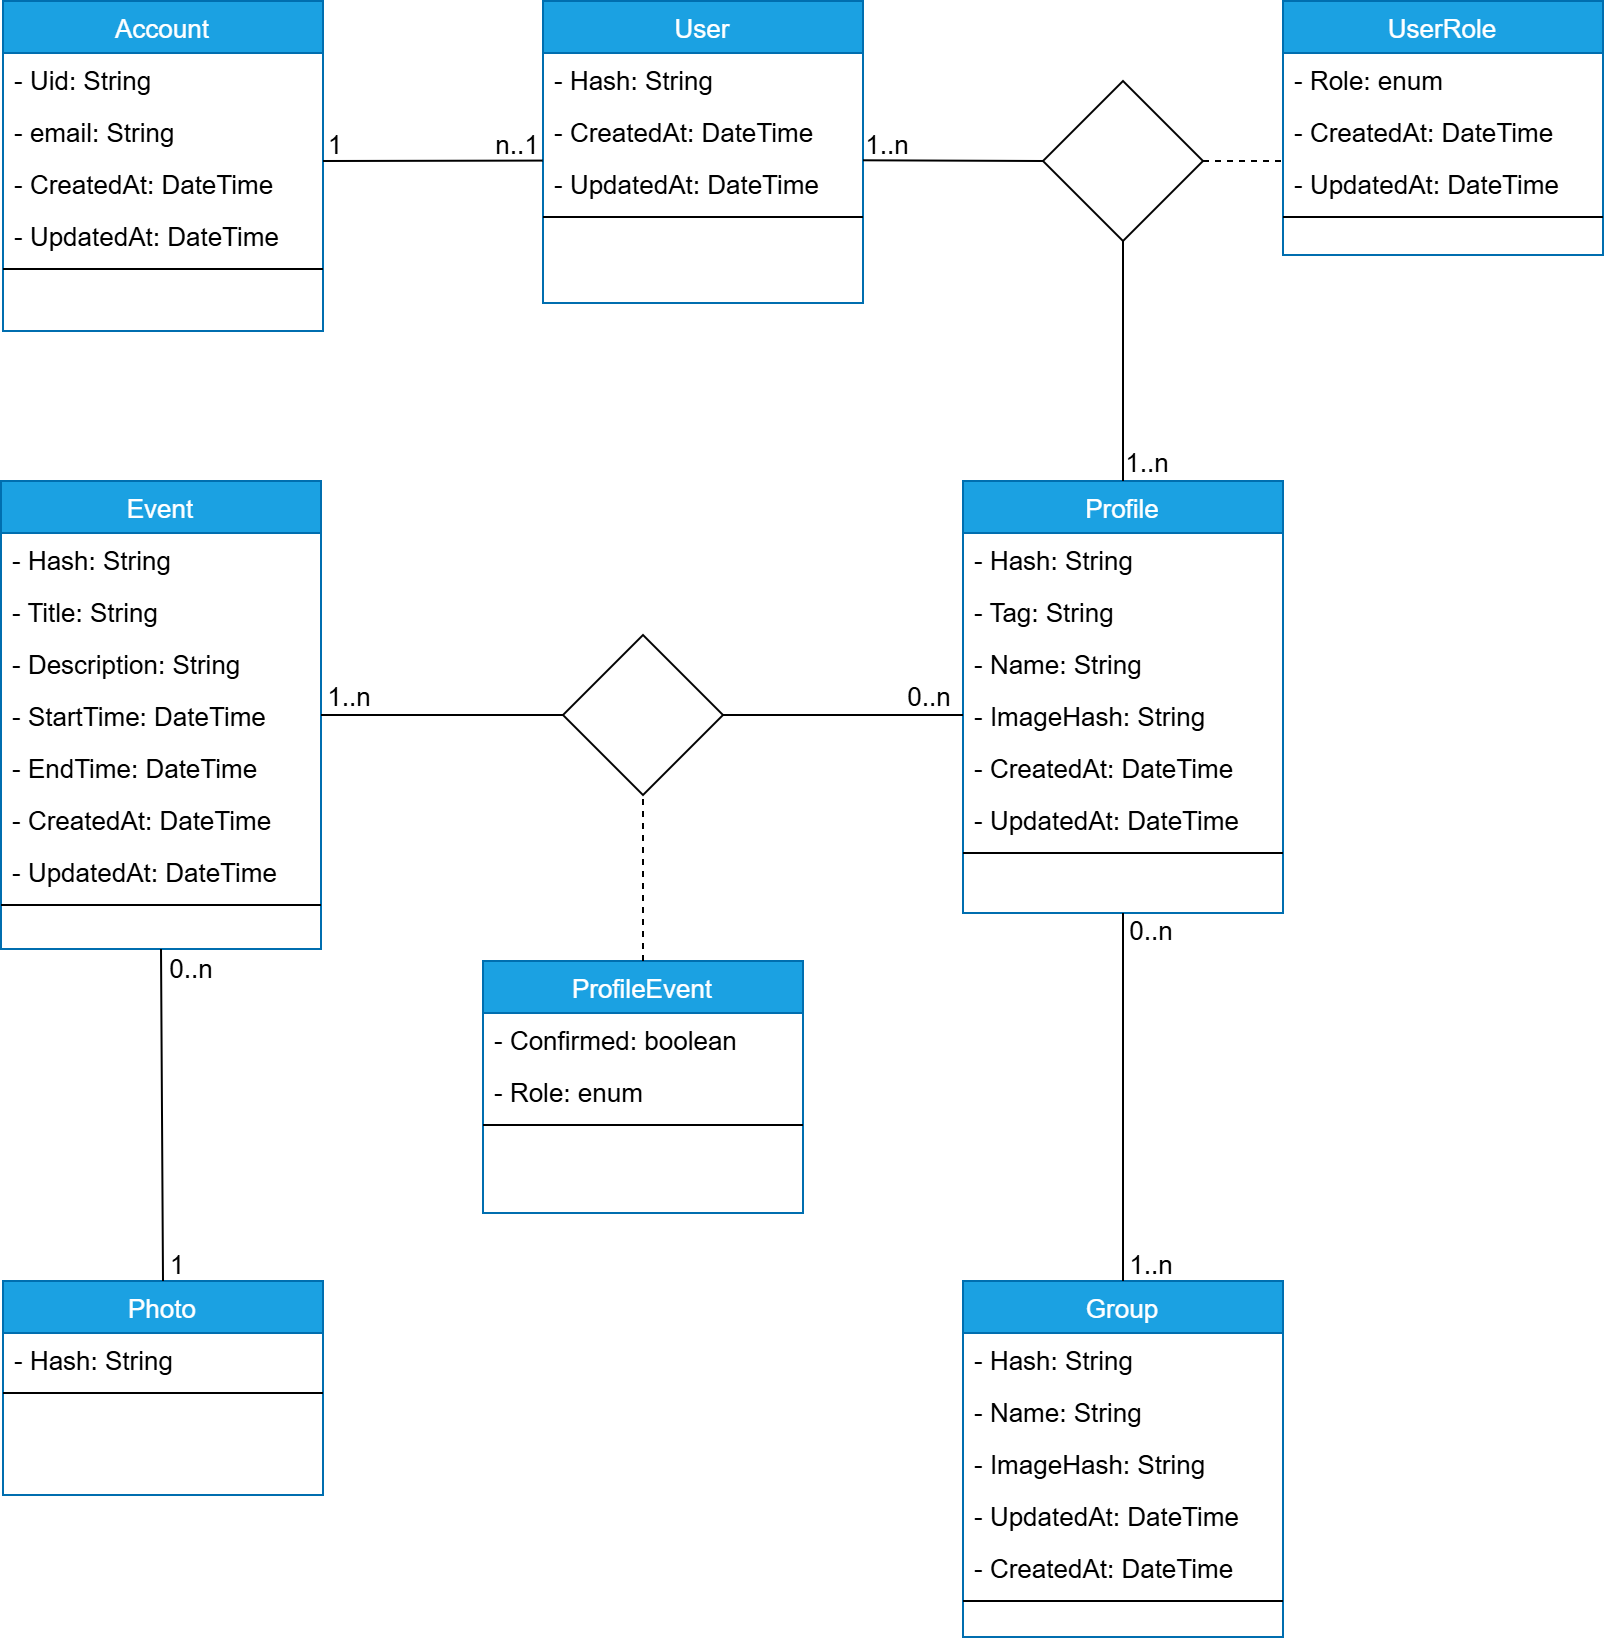
\includegraphics[width=\textwidth]{ProgettoDominioServer.png}
    \caption{Diagramma del dominio}
\end{figure}
Le richieste riguardo alle informazioni tra Account, User e Profile, con i relativi UserRole, vengono eseguite all’avvio del programma, per poi essere mantenute in memoria locale. 
Le modifiche a questi elementi sono sporadiche.
Allo stesso modo gli oggetti Group vengono recuperati solo all’avvio dell’applicazione, e, salvo rari aggiornamenti, non occupano ulteriormente lo spazio delle richieste.\\
\\
La maggioranza delle richieste verterà sull’ottenimento dei dati relativi agli Event e ai Profile. 
Infatti ad ogni avvio dell’applicazione sarà richiesto di recuperare gli eventi di ogni profilo, mentre, ogni volta che si apre il dettaglio di un evento, 
sarà necessario recuperare i rispettivi dati, includendo i profili associati. 
Si prevede che la cardinalità dei profili associati ad un evento risieda nell’ordine delle decine, 
mentre agli eventi che si associano ai profili l’ordine di grandezza previsto risiede nelle migliaia. \\
\\

La relazione che accomuna Event e Profile è di tipologia molti a molti, identificata con l’oggetto ProfileEvent. 
L’elemento ProfileEvent, oltre a descrivere la relazione, contiene la proprietà Confirmed, che indica la conferma di partecipazione di un profilo ad un evento. 
Vista la natura del progetto, la proprietà Confirmed, assieme ai dati degli Event, sarà tra i campi che subiranno modifiche con maggiore frequenza.\\
\\
Riassumendo, le operazioni principali che vertono sulle prestazioni del database sono il recupero degli eventi relativi ai profili, il recupero dei profili collegati agli eventi, 
l’aggiornamento dei campi degli oggetti Event e la modifica del campo Confirmed relativa ai ProfileEvent.\\
\\

Nonostante sia più probabile che venga richiesto il dettaglio di un evento, e quindi sia più frequente il dover recuperare i Profile relativi all’Event, 
la proporzione delle richieste prevista non giustifica lo sbilanciamento della relazione sugli Event.
Infatti, se si salvassero tutti i ProfileEvent sull’oggetto Event, le richieste degli eventi appartenenti ai profili, sebbene meno frequenti, 
richiederebbero l’ispezione di tutti gli Event alla ricerca del Profile indicato. 
Infine, se si duplicasse l’oggetto ProfileEvent, oltre che nella sua tabella originaria, anche sugli Event la sua creazione, 
la sua eliminazione e la modifica del campo Confirmed richiederebbero il doppio delle scritture.\\
\\
Vista quindi la necessità di letture frequenti da entrambe le parti di una relazione molti a molti e la necessità di scrittura dell’oggetto che la identifica, 
si individua in un database relazionale la soluzione più efficace per il dominio del progetto. 
Infatti, i database relazionali sono ottimizzati sulle operazioni di unione tra tabelle, garantendo velocità di recupero in lettura da entrambe le parti. 
Permettendo la separazione delle tabelle e gestendo gli oggetti ProfileEvent come entità indipendenti, 
la modifica del campo Confirmed comporta il blocco del solo elemento ProfileEvent. 
Le caratteristiche ACID forniscono inoltre uno stato centrale per tutta l’applicazione, che, 
per quanto non strettamente necessario, garantisce l’uniformità delle informazioni per tutti gli utenti.\\
\\

\clearpage
\section{La scelta del database}

Azure offre un’ampia scelta di database relazionali che possono essere integrati con il resto dell’ecosistema. 
Oltre alla tecnologia proposta, nella scelta del database più adatto bisogna considerare soprattutto l’integrazione con servizi accessori, 
le particolarità del server su cui viene eseguito, e i costi che si andrà ad affrontare.\\
\\
\begin{figure}[h!]
    \centering
    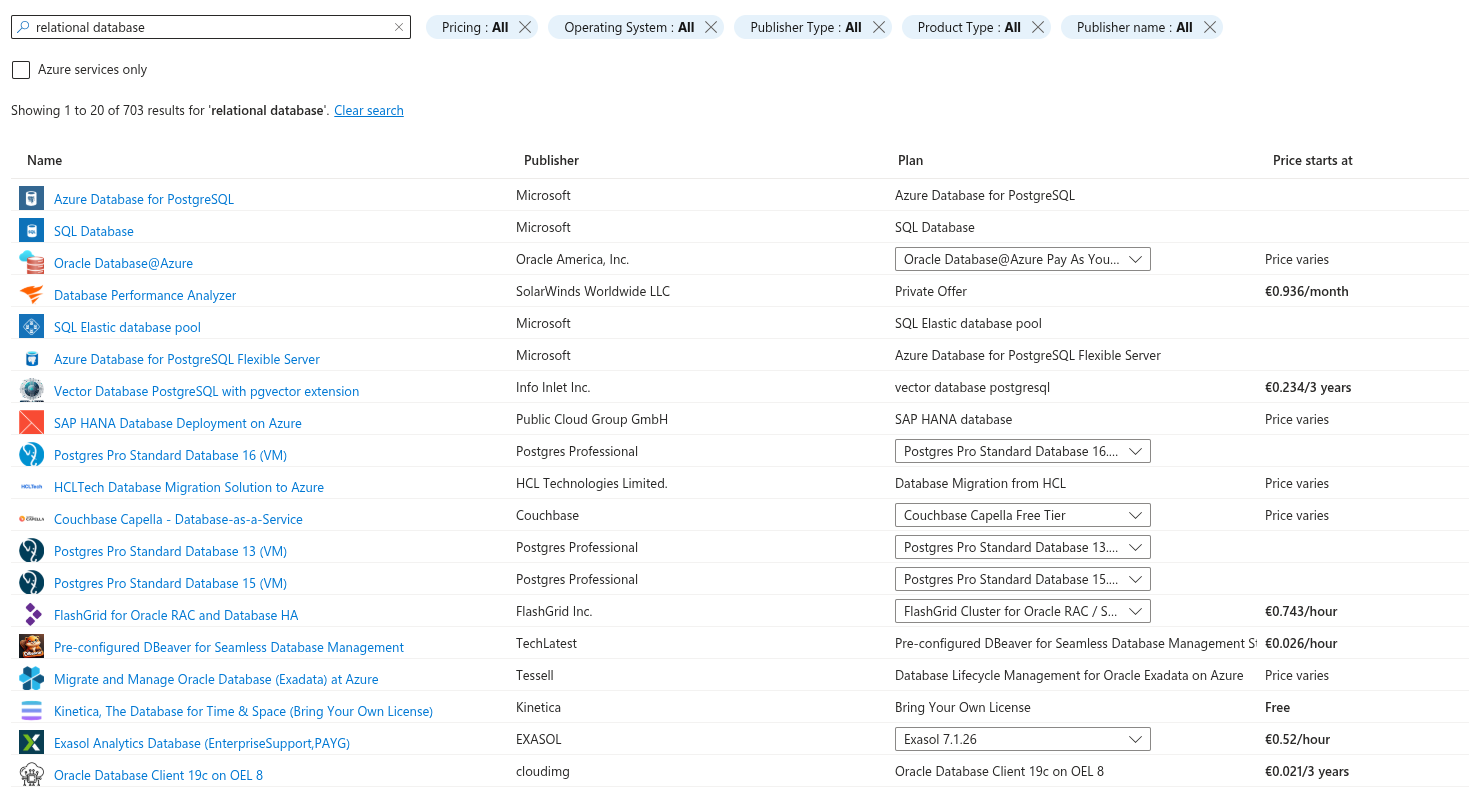
\includegraphics[width=\textwidth]{Possibilitadelcloud.png}
    \caption{Proposte di Azure per i database relazionali}
\end{figure}	


A meno di necessità particolari che richiedono l’utilizzo di una tecnologia implementata da uno specifico database, 
la grande sovrapposizione di funzionalità delle diverse offerte di database relazionali presenti sul mercato garantisce 
il  soddisfacimento delle necessità rilevate dall’analisi del dominio indipendentemente dalla tecnologia proposta dal servizio.\\
\\
La grande differenza tra i vari servizi sta nelle proprietà del server incaricato di fornire il potere computazionale necessario per l’esecuzione. 
L’architettura del server e la sua integrazione con la tecnologia del database, infatti, determinano l’effettiva capacità di scalabilità del servizio.\\
\\
Si intende scalabilità verticale la capacità di aumentare le risorse della stessa macchina in cui si esegue il codice. 
La scalabilità verticale viene definita nel momento di creazione del servizio, in cui si determinano le risorse da dedicare alla macchina che esegue il programma. 
Trattandosi di macchine virtualizzate, è sempre possibile in un secondo momento aumentare le prestazioni in caso di necessità.\\
\\

Per scalabilità orizzontale si intende invece la capacità di delegare il carico di lavoro ad altre macchine, eventualmente coordinando le modifiche. 
Questo permette una risposta alle richieste più resistente, riducendo il rischio di colli di bottiglia che potrebbero venirsi a formare nell’utilizzo di un nodo singolo.
La scalabilità orizzontale richiede però l’implementazione di tecnologie apposite integrate con il database che permettano l’esecuzione in nodi fisici differenti. \\
\\
Una volta individuata la tecnologia adatta e il livello di scalabilità desiderati, 
è bene considerare le altre necessità o le opportunità aggiuntive generate dalla presenza di un database nel progetto. \\
\\

L’alta disponibilità(HA) è la proprietà di garantire l’accesso al servizio nonostante i guasti. 
Ad esempio, si può mantenere una macchina identica al server principale in grado di replicare il servizio, spostando il carico in caso di guasto del server principale. 
Si misura in “numero di nove”, ovvero la quantità di nove presenti nella percentuale del tempo per il quale si garantisce la disponibilità del servizio.
I servizi offrono diverse qualità di HA, in base alle funzionalità desiderate.\\
\\

Alcuni servizi possono presentare offerte di backup per riportare il server nello stesso stato di qualche momento precedente. 
Questo permette il ripristino del sistema ad un punto precedente rispetto all’avvenimento di eventuali errori o guasti del sistema.\\
\\

Inoltre, Azure mette a disposizione molteplici servizi accessori che possono essere uniti al servizio. 
Questo permette di estendere le potenzialità del database tramite  l’analisi e il monitoraggio dei dati, 
generando prestazioni aggiuntive o integrando i dati per lo sviluppo di altre tecnologie.\\
\\
Infine è necessario controllare i costi che le scelte progettuali e prestazionali hanno comportato: 
pur generalmente legati al consumo effettivo delle risorse, e quindi in grado di fornire solo una previsione del costo finale, 
ogni decisione presa conduce ad un possibile aumento di prezzo, 
ed è quindi bene controllare che le risorse selezionate siano effettivamente  necessarie a soddisfare i requisiti del progetto.\\
\\
Riducendo al minimo i costi, visto l’utilizzo iniziale dell’applicazione, e nessuna necessità tecnologica specifica, 
la scelta del database per la persistenza del progetto è ricaduta su Azure SQL Database. 
Presentando un database relazionale di tecnologia proprietaria di Microsoft, Azure SQL database esegue su un solo nodo, 
fornendo però la possibilità di  scalare  verticalmente tramite la possibilità di modificare le risorse assegnate in ogni momento, 
garantendo comunque prestazioni soddisfacenti per il servizio.\\
\\
Al server principale è stata affiancata una replica che rimane costantemente aggiornata. 
Situata in una località differente dal server principale, garantisce alta disponibilità continuando a fornire i servizi anche in caso di malfunzionamenti al server principale.
\clearpage

Nel caso in cui però fossero necessarie ulteriori prestazioni, 
se il dominio e i requisiti lo permettono, 
si può eventualmente delegare a un database non relazionale le modifiche ai dati e alle relazioni 
che non necessitano delle qualità ACID ma richiedono un’alta frequenza di scrittura.\\
\\ 
Per ovviare ai problemi di scalabilità alcune soluzioni e accortezze
possono essere adottate per migliorarne le prestazioni. 
Sicuramente si deve limitare al minimo il tempo in cui ogni richiesta necessita della connessione ai dati, 
distinguendo nel codice momenti precisi e definiti in cui vengono richieste le modifiche al database. \\
\\  
Interporre una cache tra la logica applicativa e il database
semplifica e riduce il numero di richieste verso il database. 
Il livello di caching si occupa di gestire le richieste al database 
fornendo e duplicando le risposte che possiede già in memoria, 
eventualmente concentrando le richieste in caso i dati siano invece da recuperare. 
Per i dati in scrittura, invece, salva temporaneamente le modifiche richieste, 
aggiornando subito la memoria locale, 
per poi apportare le modifiche al database in momenti di carico ridotto. 
Garantisce così un tempo di risposta e di propagazione degli aggiornamenti ridotto,
alleviando il numero di richieste al database, estendendo così  le prestazioni fornite.\\
\\


Tuttavia, non vi è alcun vincolo che impedisca l'affiancamento di database di tipologia diversa 
per rispondere a esigenze specifiche e sfruttare i punti di forza di entrambe le tecnologie.
\\


\subsection{L' integrazione con C\#}

La scelta di un database relazionale per la persistenza ha comportato sviluppi progettuali precisi. 
In primis si rende necessario tradurre il dominio in componenti relazionali che possano essere espressi e salvati nelle tabelle del database.

\begin{figure}[h!]
    \centering
    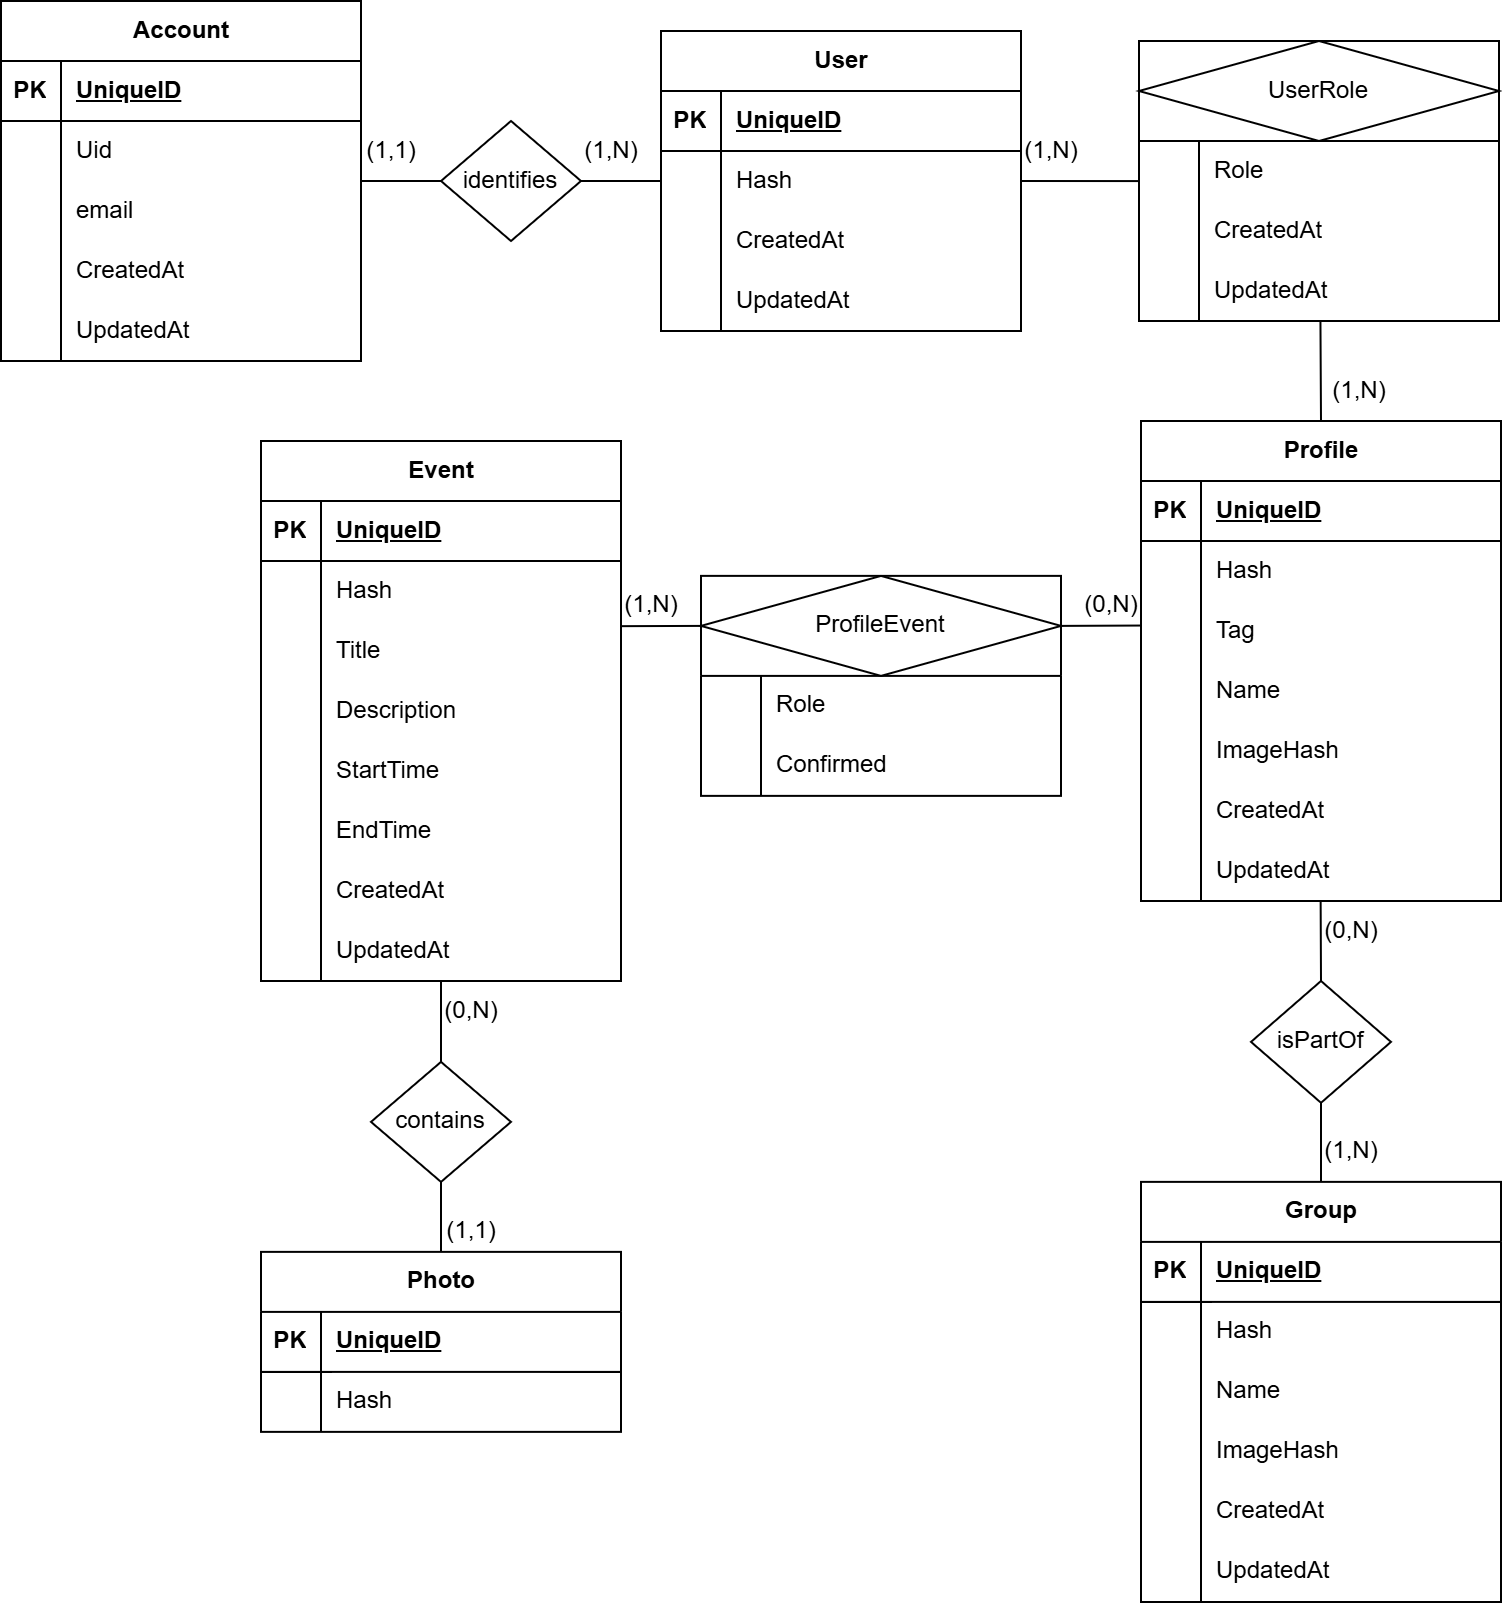
\includegraphics[width=\textwidth]{ProgettoDiagrammaER.png}
    \caption{Diagramma Entità - Relzione del dominio}
\end{figure}	

Si creano quindi sul server le classi logiche del programma, a partire dal dominio. 
Ogni classe corrisponde ad un oggetto del dominio, presentando i valori e le relazioni dei componenti come attributi dell’oggetto.\\
\\
Entity Framework Core di .Net(EFCore) è una libreria di C\# che permette di unire le classi logiche del programma alle tabelle del database. 
Fornisce un’astrazione logica del collegamento con il database e le richieste relative, fornendo una rappresentazione di alto livello delle connessioni sottostanti. \\
\\
Una volta collegato il server con il database tramite le stringhe di connessione salvate sull’Azure Key Vault, 
sono state definite le proprietà tra le varie entità, per poi inizializzare in automatico la struttura del database. 
Le modifiche alla struttura del database vengono infatti generate automaticamente da EFCore in seguito alla creazione o alla modifica degli attributi degli oggetti. 
Questo permette di star dietro agli aggiornamenti, generando e salvando le modifiche da applicare ad ogni modifica delle proprietà del dominio.\\
\\
\begin{figure}[h!]
    \begin{center}
        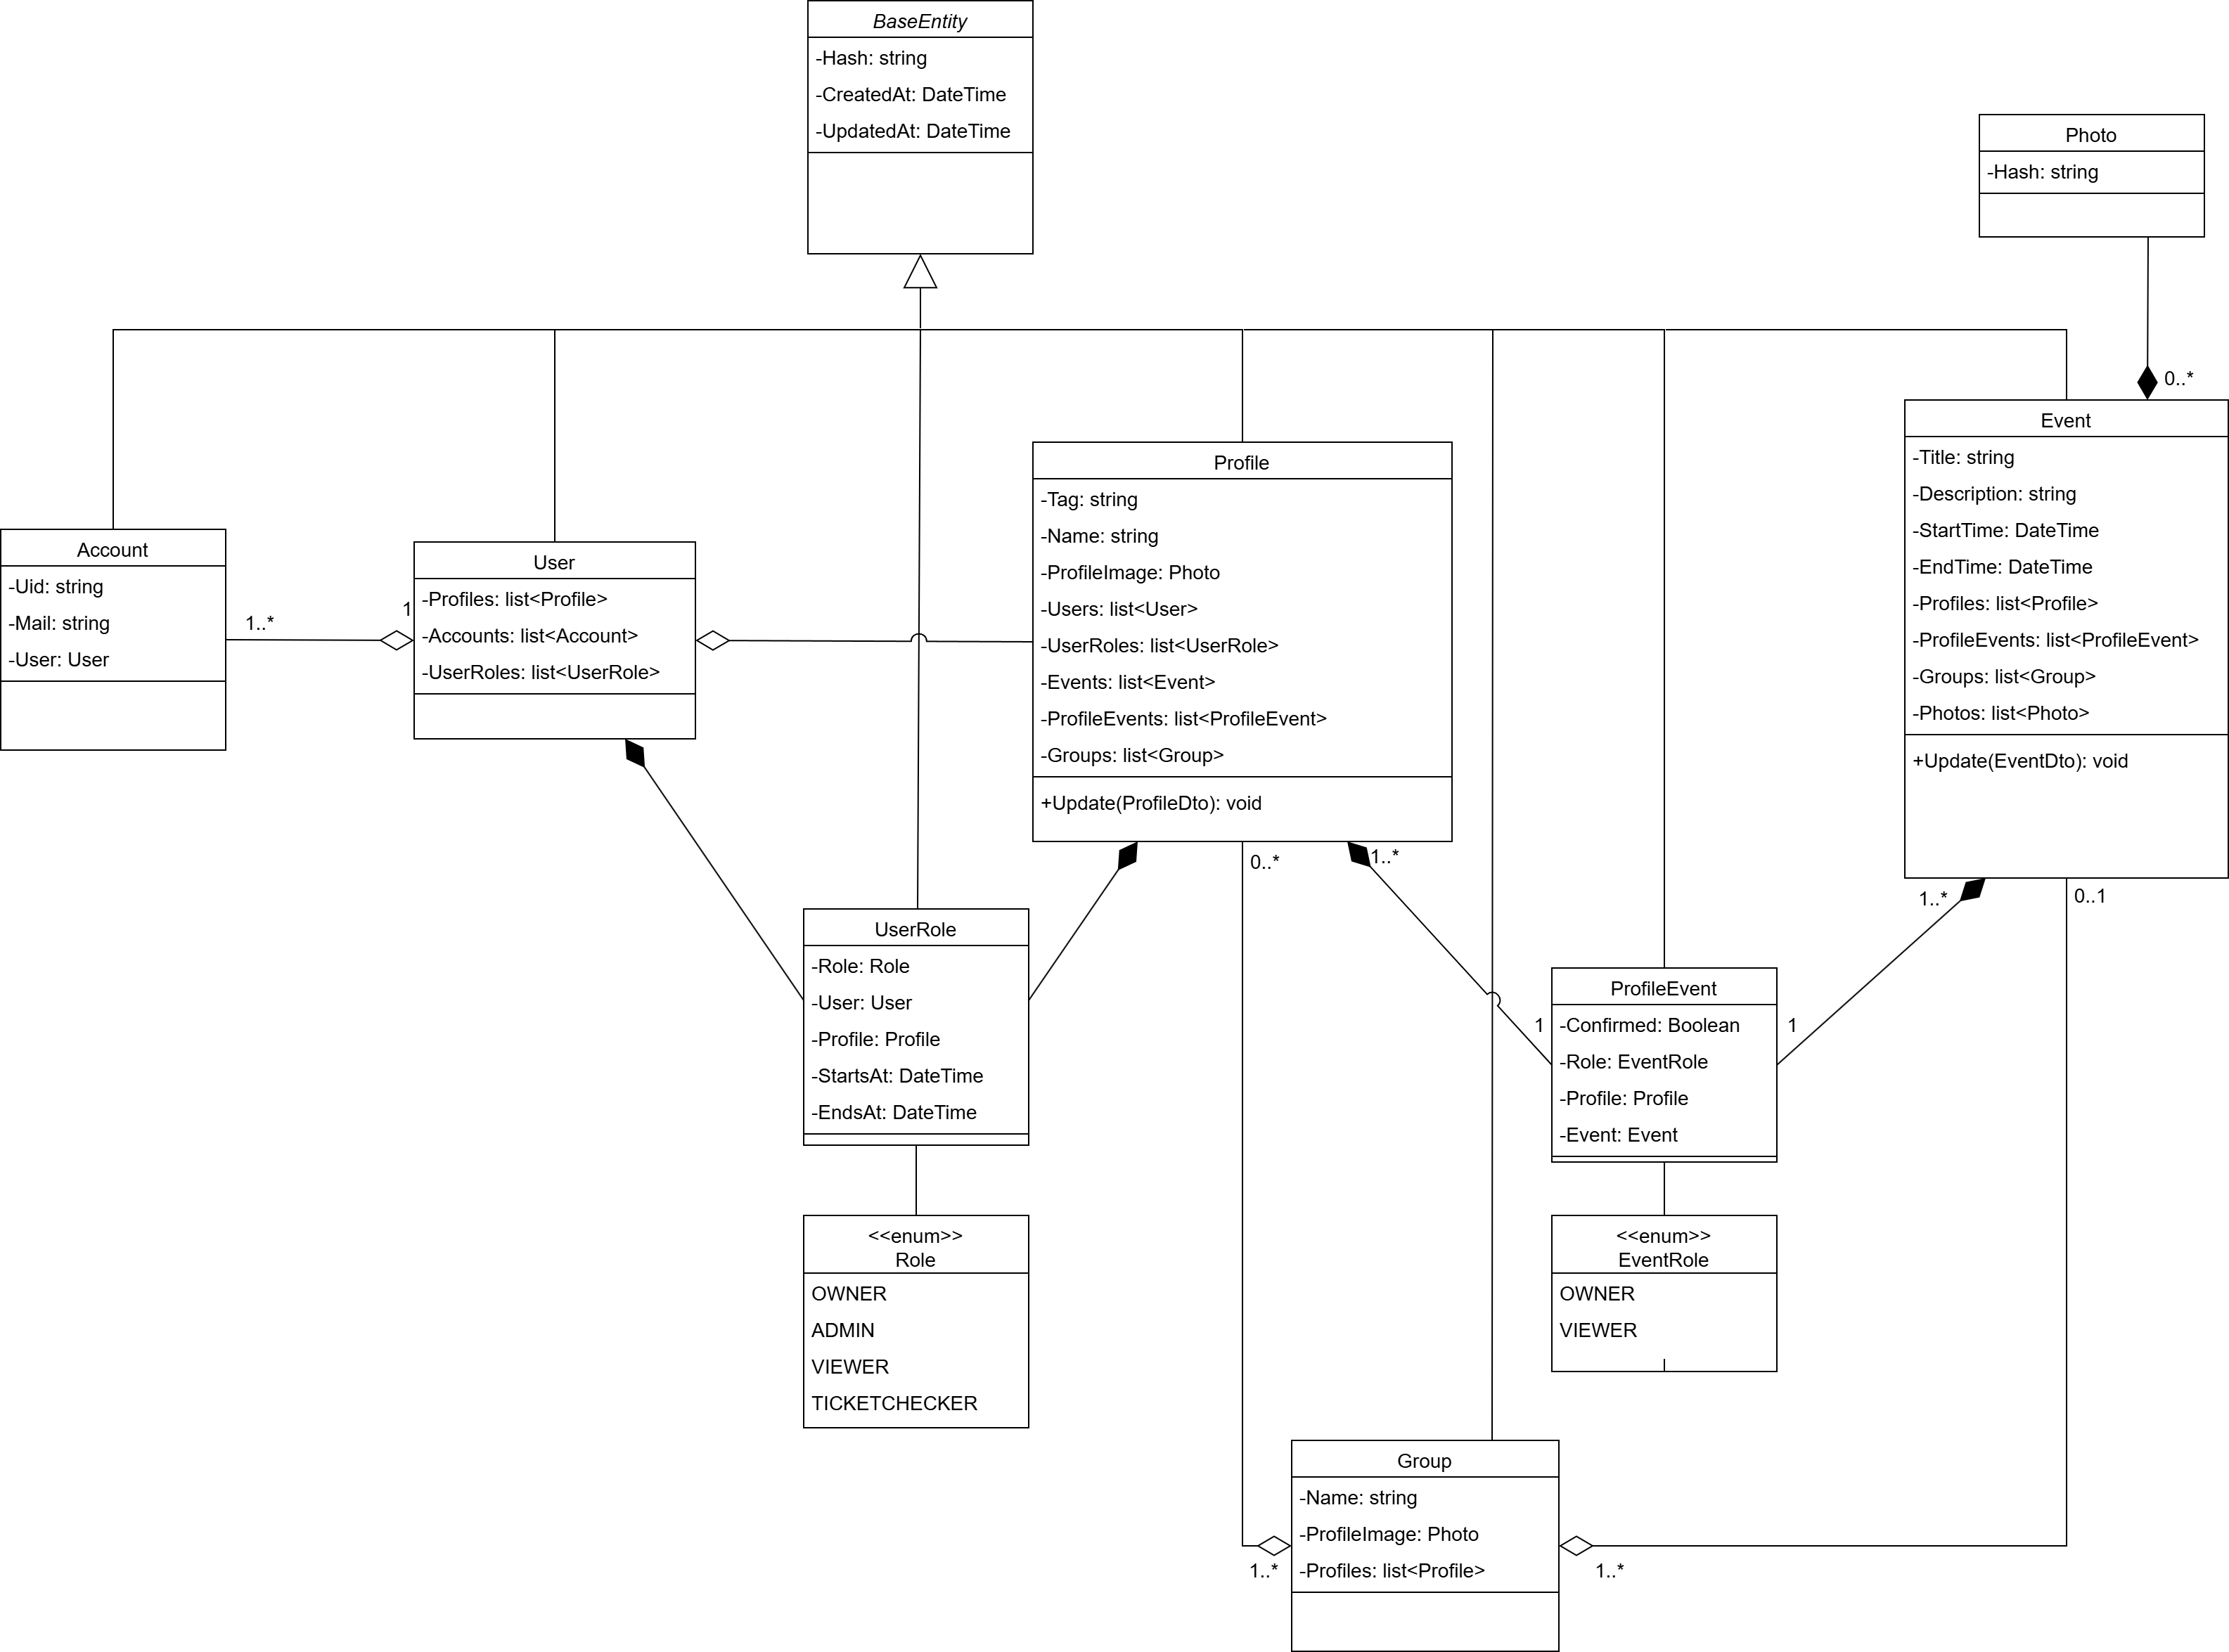
\includegraphics[width=\textwidth]{ModelClassDiagram.png}
        \caption{Modello delle classi del client}
    \end{center}
\end{figure}

Per la riduzione del carico computazionale richiesto da elementi con tante relazioni si utilizza la tecnica del lazy loading. 
La tecnica del Lazy Loading consiste nel richiedere i dati delle relazioni di un elemento solo quando strettamente necessario. 
La sua realizzazione tramite EFCore è attuata grazie alla proprietà virtual, 
che permette di gestire un oggetto con un riferimento al database richiedendo i dati delle sue relazioni solo quando viene espressamente richiesto.
\clearpage